\chapter{Implementacija i korisničko sučelje}
		
		
		\section{Korištene tehnologije i alati}
		
			\textbf{\textit{dio 2. revizije}}
			
			 \textit{Detaljno navesti sve tehnologije i alate koji su primijenjeni pri izradi dokumentacije i aplikacije. Ukratko ih opisati, te navesti njihovo značenje i mjesto primjene. Za svaki navedeni alat i tehnologiju je potrebno \textbf{navesti internet poveznicu} gdje se mogu preuzeti ili više saznati o njima}.
			
			
			\eject 
		
	
		\section{Ispitivanje programskog rješenja}
					
			\subsection{Ispitivanje komponenti}
			\textit{Potrebno je provesti ispitivanje jedinica (engl. unit testing) nad razredima koji implementiraju temeljne funkcionalnosti. Razraditi \textbf{minimalno 6 ispitnih slučajeva} u kojima će se ispitati redovni slučajevi, rubni uvjeti te izazivanje pogreške (engl. exception throwing). Poželjno je stvoriti i ispitni slučaj koji koristi funkcionalnosti koje nisu implementirane. Potrebno je priložiti izvorni kôd svih ispitnih slučajeva te prikaz rezultata izvođenja ispita u razvojnom okruženju (prolaz/pad ispita). }
			
			
			
			\subsection{Ispitivanje sustava}
			
			Ispitivanje sustava ostvareno je korištenjem Selenium WebDrivera i programskog jezika Python. U nastavku su opisani provedeni testovi, te su priloženi kodovi.
			
			U prvom ispitnom slučaju ispitan je pokušaj prijave s emailom koji nije povezan niti jedan račun, tj. emailom koji ne postoji u sustavu. Očekivani izlaz je neuspjeh pri pokušaju prijave.
			
			\begin{lstlisting}[language=Python, breaklines=true]
def test1() -> bool:
    driver = webdriver.Firefox()
    driver.get("http://localhost:3000/login")
    driver.find_element_by_name("username").send_keys("stanovnik@stanovnik.com")
    driver.find_element_by_name("password").send_keys("stanovnik")
    driver.find_element_by_css_selector("button[type='submit']").click()
    try:
        driver.find_element_by_class_name("logout")
    except NoSuchElementException:
        driver.close()
        return True
    driver.close()
    return False		
			\end{lstlisting}

			U drugom ispitnom slučaju ispitan je pokušaj registracije s neispravnim podacima, konkretno s emailom koji je zadan u krivom formatu. Očekivani izlaz je neuspjeh pri pokušaju registracije.
		
			\begin{lstlisting}[language=Python, breaklines=true]
def test2() -> bool:
    driver = webdriver.Firefox()
    driver.get("http://localhost:3000/login")
    driver.find_element_by_css_selector("button[type='button']").click()
    driver.find_element_by_name("firstname").send_keys("Stanovnik")
    driver.find_element_by_name("lastname").send_keys("Stanovnikic")
    driver.find_element_by_name("username").send_keys("stanovnik")
    driver.find_element_by_name("password").send_keys("stanovnik")
    dropdown = driver.find_element_by_class_name("css-tlfecz-indicatorContainer")
    dropdown.click()
    actions = ActionChains(driver)
    actions.move_to_element(dropdown).send_keys("Ulica 1 Kvarta 1").key_down(Keys.ENTER).key_up(Keys.ENTER).perform()
    driver.find_element_by_name("streetnumber").send_keys("7")
    driver.find_element_by_css_selector("button[type='submit']").click()
    try:
        driver.find_element_by_class_name("logout")
    except NoSuchElementException:
        driver.close()
        return True
    driver.close()
    return False
			\end{lstlisting}
			
			U trećem ispitnom slučaju ispitan je pokušaj registracije gdje su svi uneseni podaci valjani. Očekivani izlaz je uspjeh pri pokušaju registracije i preusmjeravanje na početnu stranicu korisnikovog kvarta.
			
			\begin{lstlisting}[language=Python, breaklines=true]
def test3() -> bool:
    driver = webdriver.Firefox()
    driver.get("http://localhost:3000/login")
    driver.find_element_by_css_selector("button[type='button']").click()
    driver.find_element_by_name("firstname").send_keys("Stanovnik")
    driver.find_element_by_name("lastname").send_keys("Stanovnikic")
    driver.find_element_by_name("username").send_keys("stanovnik@stanovnik.com")
    driver.find_element_by_name("password").send_keys("stanovnik")
    dropdown = driver.find_element_by_class_name("css-tlfecz-indicatorContainer")
    dropdown.click()
    actions = ActionChains(driver)
    actions.move_to_element(dropdown).send_keys("Ulica 1 Kvarta 1").key_down(Keys.ENTER).key_up(Keys.ENTER).perform()
    driver.find_element_by_name("streetnumber").send_keys("7")
    driver.find_element_by_css_selector("button[type='submit']").click()
    try:
        driver.find_element_by_class_name("logout")
    except NoSuchElementException:
        driver.close()
        return False
    driver.close()
    return True	
			\end{lstlisting}
			
			U četvrtom ispitnom slučaju ispitan je pokušaj prijave s emailom za koji postoji korisnički račun, ali s neispravnom lozinkom. Očekivani izlaz je neuspjeh pri pokušaju prijave.
			
			\begin{lstlisting}[language=Python, breaklines=true]
def test4() -> bool:
    driver = webdriver.Firefox()
    driver.get("http://localhost:3000/login")
    driver.find_element_by_name("username").send_keys("stanovnik@stanovnik.com")
    driver.find_element_by_name("password").send_keys("stanovni")
    driver.find_element_by_css_selector("button[type='submit']").click()
    try:
        driver.find_element_by_class_name("logout")
    except NoSuchElementException:
        driver.close()
        return True
    driver.close()
    return False
			\end{lstlisting}
			
			U petom ispitnom slučaju ispitan je pokušaj prijave gdje su svi uneseni podaci ispravni. Očekivani izlaz je uspjeh pri pokušaju prijave i preusmjeravanje na početnu stranicu korisnikovog kvarta.
			
			\begin{lstlisting}[language=Python, breaklines=true]
def test5() -> bool:
    driver = webdriver.Firefox()
    driver.get("http://localhost:3000/login")
    driver.find_element_by_name("username").send_keys("stanovnik@stanovnik.com")
    driver.find_element_by_name("password").send_keys("stanovnik")
    driver.find_element_by_css_selector("button[type='submit']").click()
    try:
        driver.find_element_by_class_name("logout")
    except NoSuchElementException:
        driver.close()
        return False
    driver.close()
    return True
			\end{lstlisting}
			
			Na slici 5.2 prikazana je snimka zaslona terminala kao rezultat izvođenja prethodno navedenih pet ispitnih slučajeva.
			
			\begin{figure}[H]
					\centering
					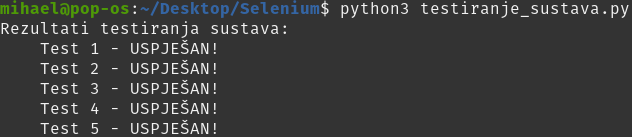
\includegraphics[width=\textwidth,keepaspectratio]{18 ispitivanje sustava.png}
					\caption{Rezultati ispitivanja Selenium WebDriverom}
				\end{figure}	
			\eject 
		
		
		\section{Dijagram razmještaja}
		
		Na slici 5.3 prikazan je dijagram razmještaja. Sustav je baziran na arhitekturi "klijent-poslužitelj". Korisnici pristupaju aplikaciji korištenjem web preglednika. Na platformi Heroku se nalaze poslužitelji za frontend, backend i bazu podataka. Komunikacija između korisnika i poslužitelja za frontend, te poslužitelja za frontend i poslužitelja za backend, ostvaruje se korištenjem protokola HTTP.
			
			\begin{figure}[H]
					\centering
					\includegraphics[width=\textwidth,keepaspectratio]{17 dijagram razmještaja.png}
					\caption{Dijagram razmještaja}
				\end{figure}	
			
			\eject 
		
		\section{Upute za puštanje u pogon}
		
			\textbf{\textit{dio 2. revizije}}\\
		
			 \textit{U ovom poglavlju potrebno je dati upute za puštanje u pogon (engl. deployment) ostvarene aplikacije. Na primjer, za web aplikacije, opisati postupak kojim se od izvornog kôda dolazi do potpuno postavljene baze podataka i poslužitelja koji odgovara na upite korisnika. Za mobilnu aplikaciju, postupak kojim se aplikacija izgradi, te postavi na neku od trgovina. Za stolnu (engl. desktop) aplikaciju, postupak kojim se aplikacija instalira na računalo. Ukoliko mobilne i stolne aplikacije komuniciraju s poslužiteljem i/ili bazom podataka, opisati i postupak njihovog postavljanja. Pri izradi uputa preporučuje se \textbf{naglasiti korake instalacije uporabom natuknica} te koristiti što je više moguće \textbf{slike ekrana} (engl. screenshots) kako bi upute bile jasne i jednostavne za slijediti.}
			
			
			 \textit{Dovršenu aplikaciju potrebno je pokrenuti na javno dostupnom poslužitelju. Studentima se preporuča korištenje neke od sljedećih besplatnih usluga: \href{https://aws.amazon.com/}{Amazon AWS}, \href{https://azure.microsoft.com/en-us/}{Microsoft Azure} ili \href{https://www.heroku.com/}{Heroku}. Mobilne aplikacije trebaju biti objavljene na F-Droid, Google Play ili Amazon App trgovini.}
			
			
			\eject 